%! Author = Daniil
%! Date = 15.05.25

\documentclass[12pt]{article}
\usepackage{pdflscape}
\usepackage{rotating} % otočení tabulky

% +-------------------+
% | Rozložení stránek |
% +-------------------+
\usepackage[
    a4paper,
    width=150mm,
%  height=220mm,
    top=25mm,
    bottom=25mm
]{geometry}


% +------+
% | Font |
% +------+
\usepackage{fontspec}
\setmainfont{Linux Libertine O}


% +---------+
% | Čeština |
% +---------+
\usepackage[czech]{babel}


% +------------------------------------+
% | programovací jazyk Lua - LuaLaTeX  |
% +------------------------------------+
\usepackage{luacode}
\newcommand{\luavar}[1]{\directlua{tex.sprint(#1)}}
\begin{luacode*}
-- vrací uživatelem zadané datum nebo aktuální datum
function get_date()
  if (date == nill or date == '') then
    return tex.print('\\today')
  else
    return tex.print(date)
  end
end

-- vrací všechny autory dokumentu( jméno + obor) naformátované pro TeX
function get_authors()
  local result = ""
  for i, author in ipairs(authors) do
    result = result .. author.name .. "&&&&&" .. author.program .. "\\\\"
  end
  return result
end

-- vrací počet autorů
function get_authors_count()
    local result = 0
    for i, author in ipairs(authors) do
        result = result + 1
    end
    return result
end

-- vrací jména všech autorů oddělená čárkami
function get_author_names()
    local result = ""
    if get_authors_count() == 1 then
        return authors[1].name
    else
        for i, author in ipairs(authors) do
            result = result .. author.name .. ", "
        end
        result = result:sub(1, -3)
        return result
    end
end

-- podmíněné výpisy
function printBiblio()
  local output = "\\newpage \\section{Literatura} \\printbibliography[heading=none]"
  if (PRINT_BIBLIO) then
    return tex.print(output)
  end
end

function printTablesList()
    if (PRINT_TABLES) then
        return tex.print("\\listoftables")
    end
end

function printFiguresList()
    if (PRINT_FIGURES) then
        return tex.print("\\listoffigures")
    end
end

function printSnippetsList()
    if (PRINT_SNIPPETS) then
        return tex.print("\\lstlistoflistings")
    end
end
\end{luacode*}


% +---------+
% | seznamy |
% +---------+
\usepackage{multicol} % vícesloupcový seznam


% +---------+
% | chemie  |
% +---------+
\usepackage{chemformula}


% +---------+
% | obrázky |
% +---------+
\usepackage{graphicx}
\graphicspath{{./images/}}
\usepackage{svg}
\usepackage{subcaption}
\usepackage{wrapfig}


% +-------+
% | barvy |
% +-------+
\usepackage{color}
\definecolor{dkgreen}{rgb}{0,0.6,0}


% +--------+
% | odkazy |
% +--------+
\usepackage{hyperref}
\hypersetup{
    colorlinks=true,
    citecolor=black,
    filecolor=black,
    linkcolor=black,
    pdftitle={\luavar{title}},
    urlcolor=teal
}

% +------------------------------+
% |         bibliografie         |
% +------------------------------+
% | používá se norma ČSN ISO 690 |
% +------------------------------+
\usepackage{csquotes}
\usepackage[style=iso-authoryear,
    hyperref=true,
    url=false,
    isbn=false,
    backref=true]{biblatex}
\addbibresource{biblio.bib}
% převedení bibliografie do kapitálek
%\renewcommand{\mkbibcompletename}[1]{\textsc{#1}}  % afektuje kromě bibliografie i citace
\renewcommand*{\mkbibnamegiven}[1]{\textsc{#1}}


% +-----------------------+
% | sazba zdrojových kódů |
% +-----------------------+
\usepackage{listings}
\renewcommand{\lstlistingname}{Zdrojový kód}
\renewcommand{\lstlistlistingname}{Seznam zdrojových kódů}

% čeština ve zdrojovém kódu
\lstset{extendedchars}
\begingroup
\catcode0=12 %
\makeatletter
\g@addto@macro\lst@DefEC{%
    \lst@CCECUse\lst@ProcessLetter
    ěščřžĚŠČŘŽťŤďĎňŇů
    ^^00%
}%
\endgroup

% stylování zdrojového kódu (barvy klíčových slov, ...)
\lstdefinestyle{mystyle}{
    backgroundcolor=\color{white},
    commentstyle=\color{dkgreen},
    keywordstyle=\color{orange},
    numberstyle=\tiny\color{gray},
    stringstyle=\color{purple},
    basicstyle=\ttfamily\footnotesize,
    breakatwhitespace=false,
    breaklines=true,
    captionpos=b,
    keepspaces=true,
    numbers=left,
    numbersep=5pt,
    showspaces=false,
    showstringspaces=false,
    showtabs=false,
    tabsize=2
}
\lstset{style=mystyle}


% +--------------------------+
% | záhlaví a zápatí stránek |
% +--------------------------+
\usepackage{fancyhdr}


% +----------------------------+
% | vlastní použitelné příkazy |
% +----------------------------+
\newcommand\lorem{
    Lorem ipsum dolor sit amet, consectetur adipiscing elit, sed do eiusmod tempor incididunt ut labore et dolore magna aliqua. Ut enim ad minim veniam, quis nostrum exercitationem ullam corporis suscipit laboriosam.
}
\newcommand\mistrjan{
    Krajani a druzi moji, ach, smutno mi je, trudno, neveselo, chmurami jsem zavalen, hanbou jsem zdrcen a jest mi za co pykat. Maje na mysli jen dobro, bez rozmyslu jsem vnesl do jazyka velkou lotrovinu a tak zavinil historickou nehodu. Dlouho se to tutlalo, teprve tato epocha celou moji vinu naplno vyjevila. Uznal jsem to a kaji se. V troufalosti ducha, a usiluje pouze o to, aby bylo lze rychleji rozmluvy, ano i knihy, skripta a lejstra zapisovati, jsem vymyslel potrhlou a krutou fintu. Brkem z husy jsem litery a, c, d, e, i, n, o, r, s, r, u, y, z pobodal a zle poranil.
}


% +-------------------+
% | Titulní stránka   |
% +-------------------+
\newcommand\mytitlepage{
    \begin{titlepage}
    \begin{center}
    \Large{
        \luavar{university}\\
        \luavar{faculty}\\
    }
    \vspace{0.2cm}
    \hrule

    \vfill
    \Huge{
        \textbf{\luavar{title}}
    }

    \vspace{1.5cm}

    \LARGE {
        \textbf{\luavar{document_type}}\\
    }

    \vspace{0.2cm}

    \Large {
        \luavar{subject}\\
    }

    \vfill

    \vspace{0.8cm}

    \Large{
        \begin{tabular}{lccccl}
        \directlua{tex.print(get_authors())}
        \end{tabular}
    }

    \vspace{1.5cm}

    \Large{
        \luavar{place}, \directlua{get_date()}
    }
    \end{center}
    \end{titlepage}
}

% +------------------------------------+
% | Nové prostředí pro vložení práce   |
% +------------------------------------+
\newenvironment{teamwork}
{% begin

% PDF meta data
    \hypersetup{
        pdfinfo={
            Title={\luavar{title}},
            Author={\luavar{get_author_names()}},
            Subject={\luavar{subject}},
            Keywords={\luavar{keywords}}
        }
    }

    % titulní stránka
    \mytitlepage

    % obsah
    \tableofcontents
    \thispagestyle{empty}
    \newpage
    \setcounter{page}{1}

    % záhlaví a zápatí
    \pagestyle{fancy}
    \fancyhead{}
    \fancyfoot{}
    \fancyhead{\nouppercase{\leftmark}\hfill\thepage}
    \setlength{\headheight}{14.5pt}
    }
    {% end

    % bibliografie
    \directlua{printBiblio()}

    % seznam obrázků
    \directlua{printFiguresList()}

    % seznam tabulek
    \directlua{printTablesList()}

    % seznam zdrojových kódů
    \directlua{printSnippetsList()}
}

% +-----------+
% | Nastavení |
% +-----------+
\begin{luacode*}
  university = "Mendelova univerzita v~Brně"
  faculty = "Provozně ekonomická fakulta"
  title = "Synchronizace obrazových a akustických dat"
  subject = "ENC-NSS: Nasazení software a služeb"
  document_type = "uživatelský manuál"
  place = "Brno"
  date = "15. 5. 2025"
  keywords = "ASS, NSS"

  -- autoři (je nutné, si hlídat abecední pořadí jmen ručně)
  authors = {}
  authors[1] = {name = "Prázdný řetězec", program = "Otevřená informatika (N-OI)"}
\end{luacode*}

% +---------------+
% | Samotná práce |
% +---------------+
\begin{document}

    \begin{teamwork}

        \section{O aplikaci}\label{sec:o-aplikace}

        Tato aplikace slouží k získávání dat o stavu rostlin ze senzorů akustické emise, RGB kamery a hyperspektrální kamery.
        V aplikaci lze po přihlášení nastavovat parametry měření, naplánovat jej na určitý den a čas, zahájit měření okamžitě, zobrazit seznam historie meření a stahovat získaná data.

        \section{Prerekvizity}\label{sec:prerekvizity}

        Je nutné, aby stroj který bude systém provozovat (a ke kterému budou připojeny senzory), splňoval určité náležitosti.
        Tento stroj musí:

        \begin{enumerate}
            \item mít nainstalované \href{https://www.ni.com/en/support/downloads/software-products/download.labview.html#559067}{LabVIEW}
            \item obsahovat síťovou kartu s alespoň dvěma Ethernet rozhraními, přičemž alespoň jedno z
            nich bude Gigabit Ethernet (připojení hyperspektrální kamery)
            \item obsahovat alespoň jeden port USB 3 (připojení RGB kamery)
            \item mít nainstalovanou řadiče a knihovnu \href{https://www.baslerweb.com/en/downloads/software/?downloadCategory.values.label.data=pylon}{Pylon od společnosti Basler (8.1.0)} (ovládání RGB kamery)
        \end{enumerate}


        \section{Přihlášení do aplikace}\label{sec:prihlaseni-do-aplikace}

        Než uživatel začne pracovat v aplikaci, je nutné se přihlásit.
        Postup je následující:

        \begin{enumerate}
            \item Na domovské stránce klikněte na tlačítko „LOG IN“
            \begin{figure}[hbt!]
                \centering
                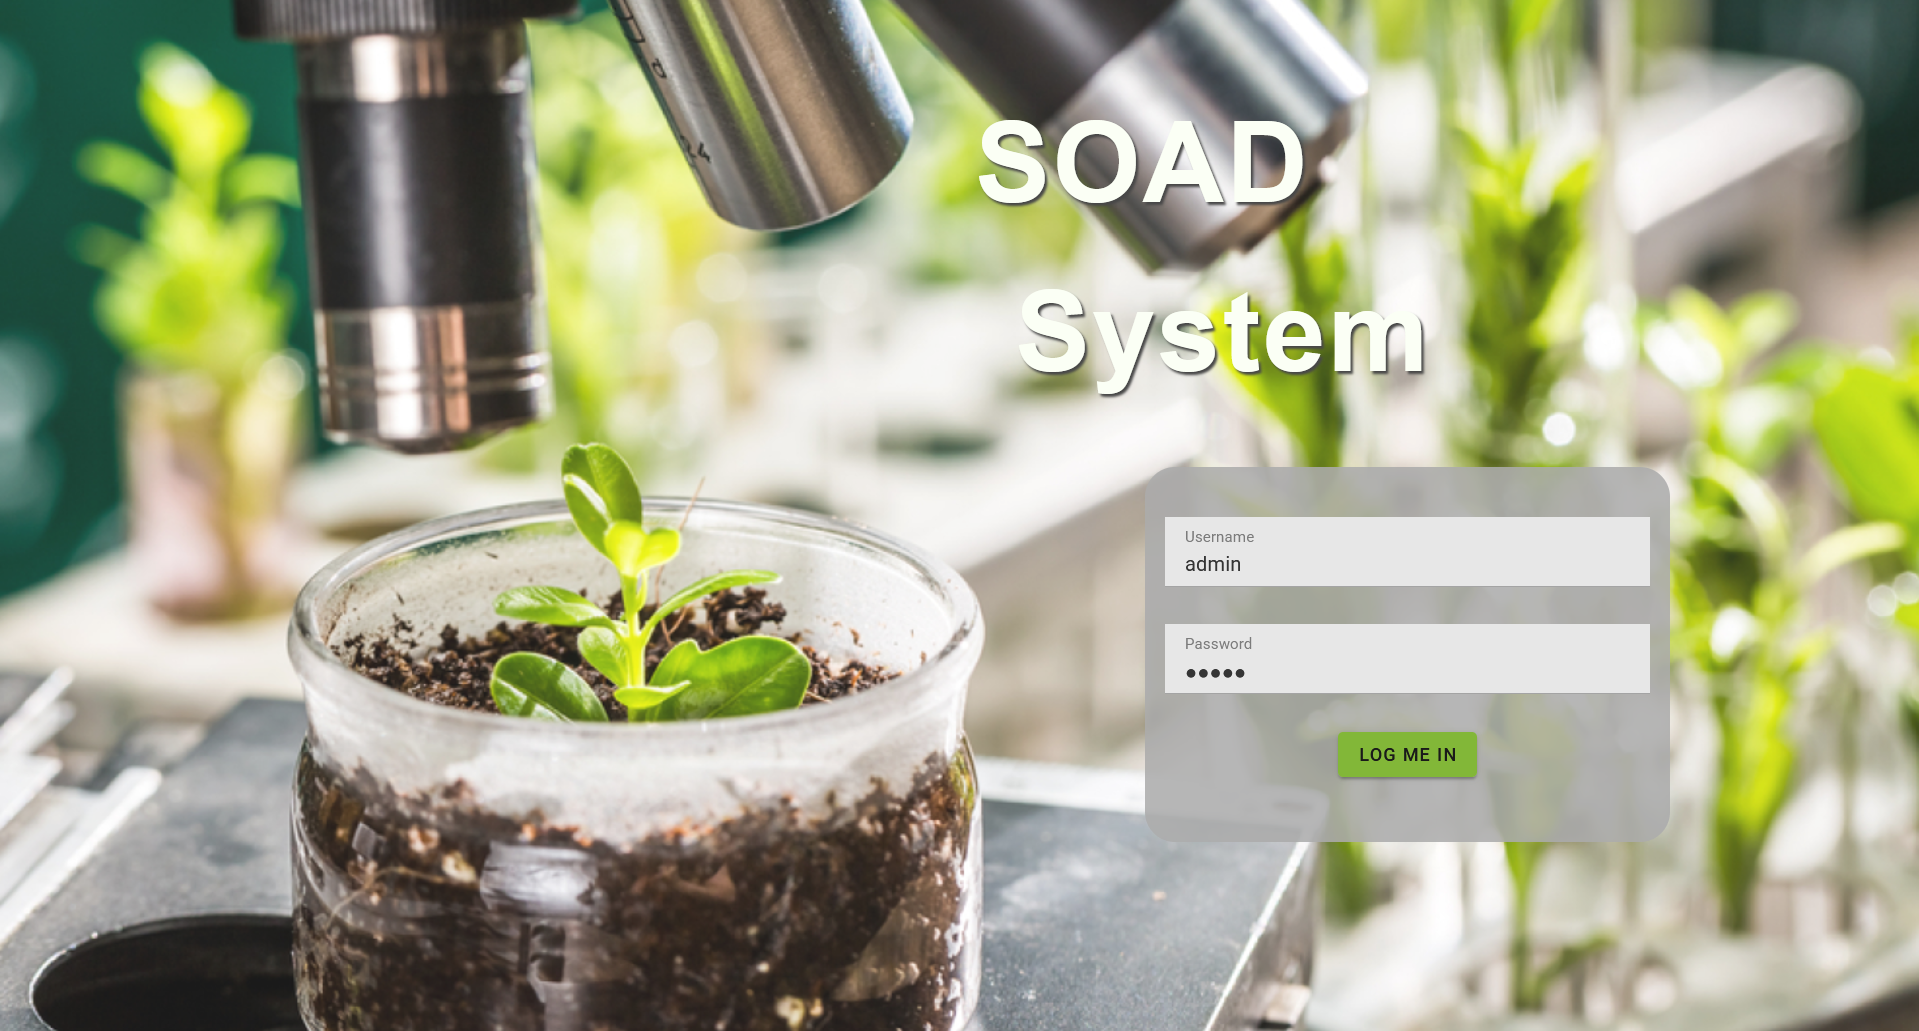
\includegraphics[width=0.8\textwidth]{../../img/main_page}
                \caption{Tlačítko pro přihlášení}
                \label{fig:tlacitko_pro_prih}
            \end{figure}
            \item Vyplňte uživatelské jméno a heslo.
            Pokud programátor použil příklad souboru \texttt{.env}, je to \textbf{admin} \textbf{admin}
            \item Přihlásíte se kliknutím na tlačítko „LOG ME IN“
            \begin{figure}[hbt!]
                \centering
                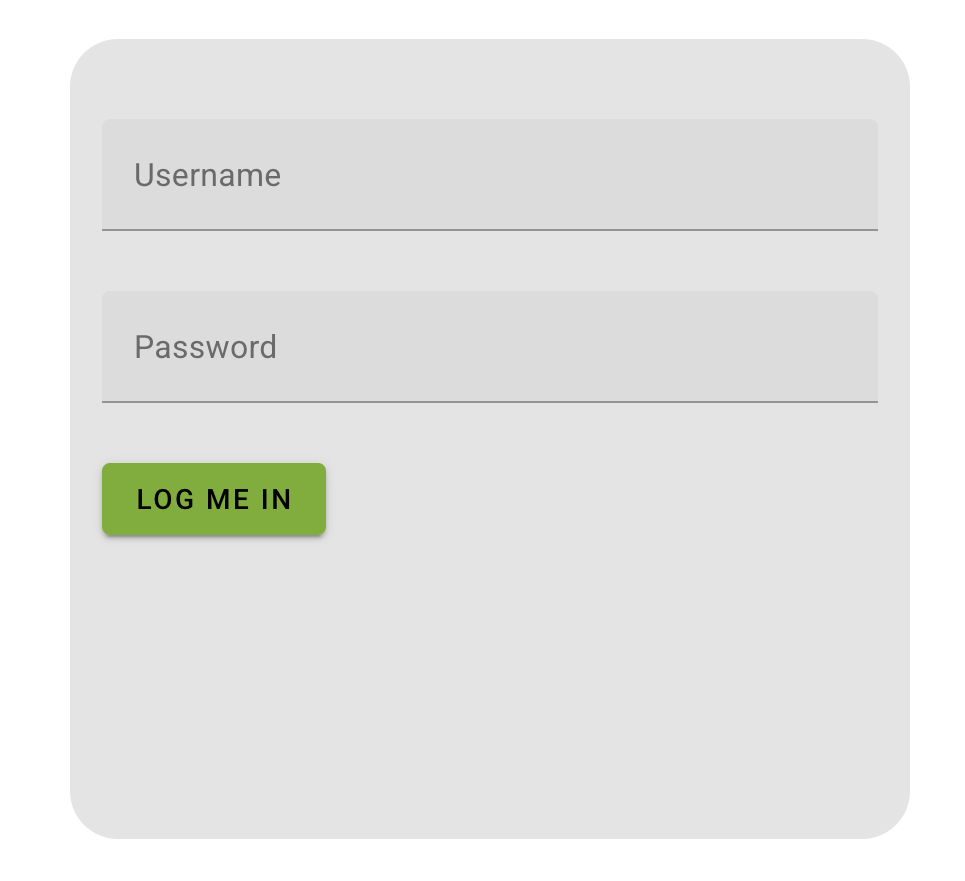
\includegraphics[width=0.45\textwidth]{../../img/login_box}
                \caption{Přihlášovací formulář}
                \label{fig:login_box}
            \end{figure}
        \end{enumerate}

        \section{Nastavení senzorů}\label{sec:nastaveni-senzoru}

        Parametry jednotlivých zařízení lze nastavit na stránce „Configuration“ (tlačítko v horní části stránky).
        Je možné upravit parametry RGB kamery, hyperspektrální kamery a zařízení na měření akustické emise.

        \subsection{RGB kamera}\label{subsec:rgb-kamera}

        Na obrázku 3 se nachází tabulka pro nastavení parametrů RGB kamery.
        U tohoto zařízení lze pomocí posuvníků
        potažením směrem vpravo či vlevo nastavit vzorkovací frekvenci a počet snímků.
        Pod nimi se nachází dvě textová
        pole, která umožňují nastavit, kdy kamera začne snímat (vlevo) a časový interval snímání (vpravo).

        \begin{figure}[hbt!]
            \centering
            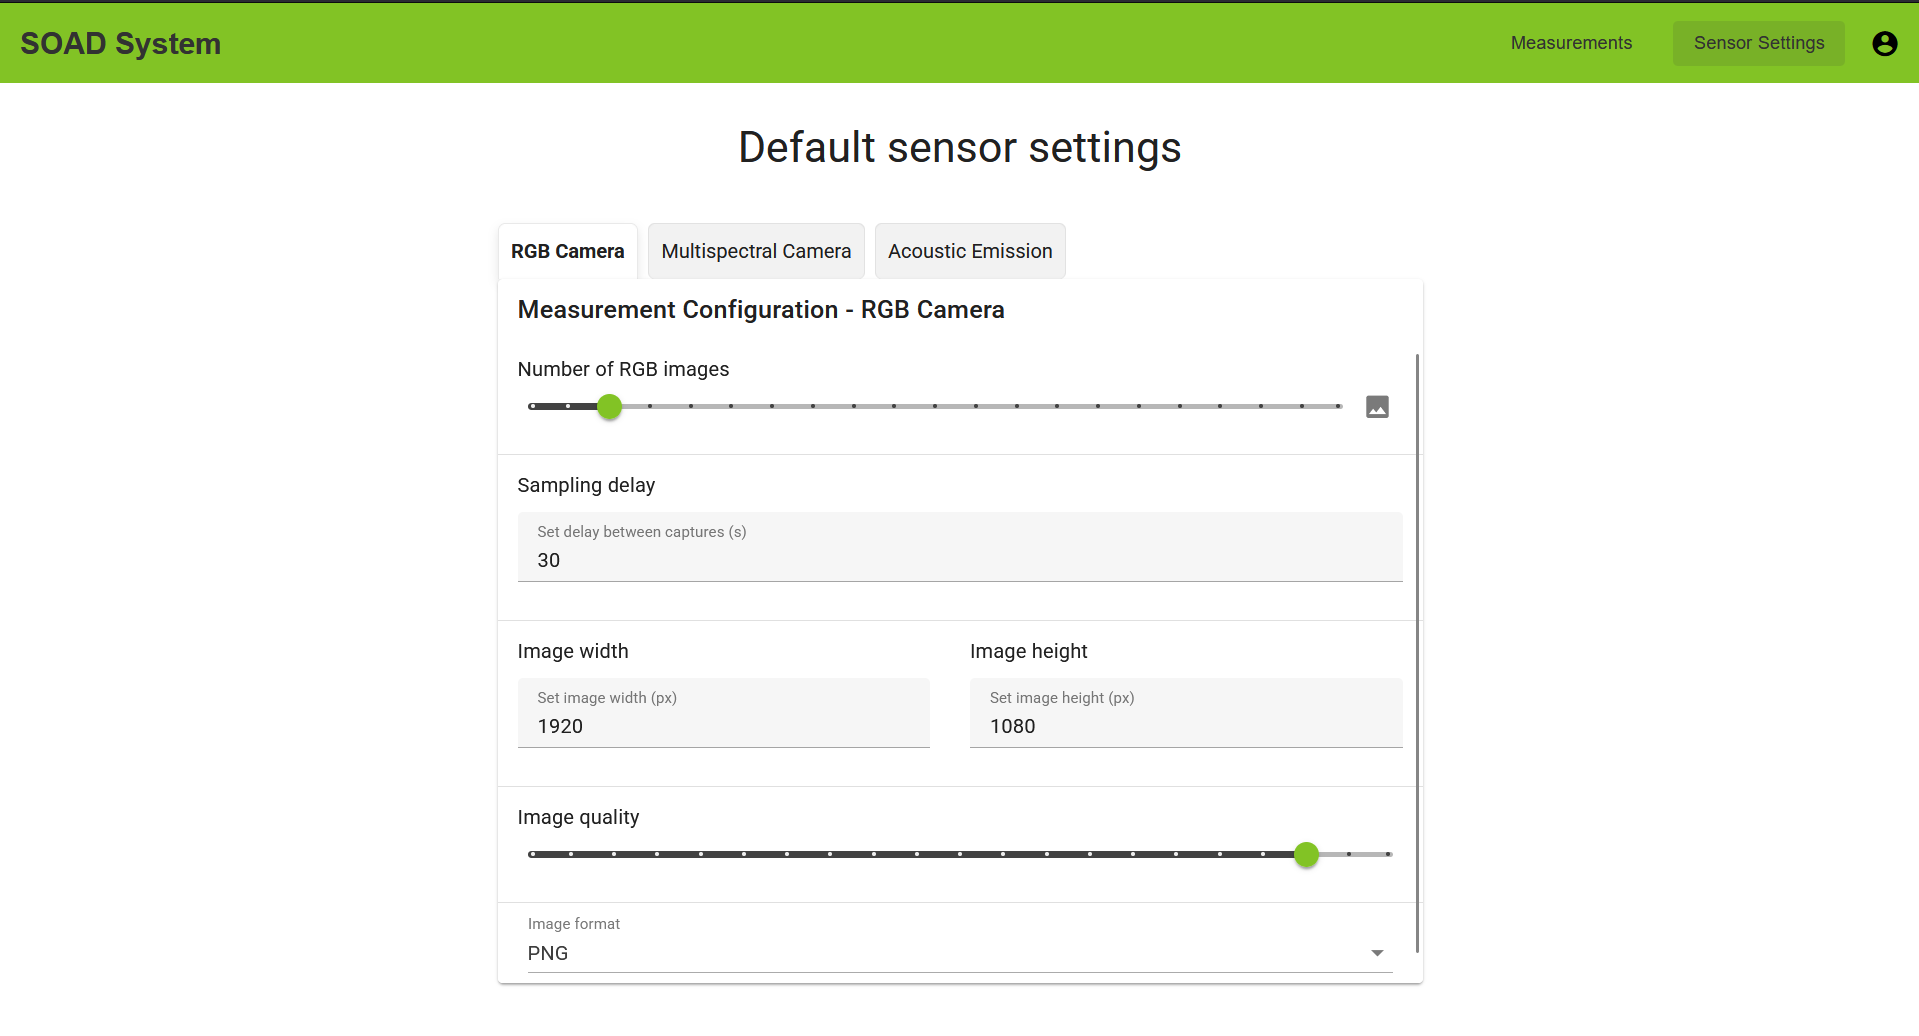
\includegraphics[width=0.7\textwidth]{../../img/rgb_cam_settings}
            \caption{Tabulka pro nastavení RGB kamery}
            \label{fig:rgb_cam_settings}
        \end{figure}

        \subsection{Hyperspektrální kamera}\label{subsec:hyperspektralni-kamera}

        Nastavení hyperspektrální kamery, které je zobrazeno na obrázku 4,
        je shodné s nastavením RGB kamery (viz předchozí sekce RGB kamera).

        \begin{figure}[hbt!]
            \centering
            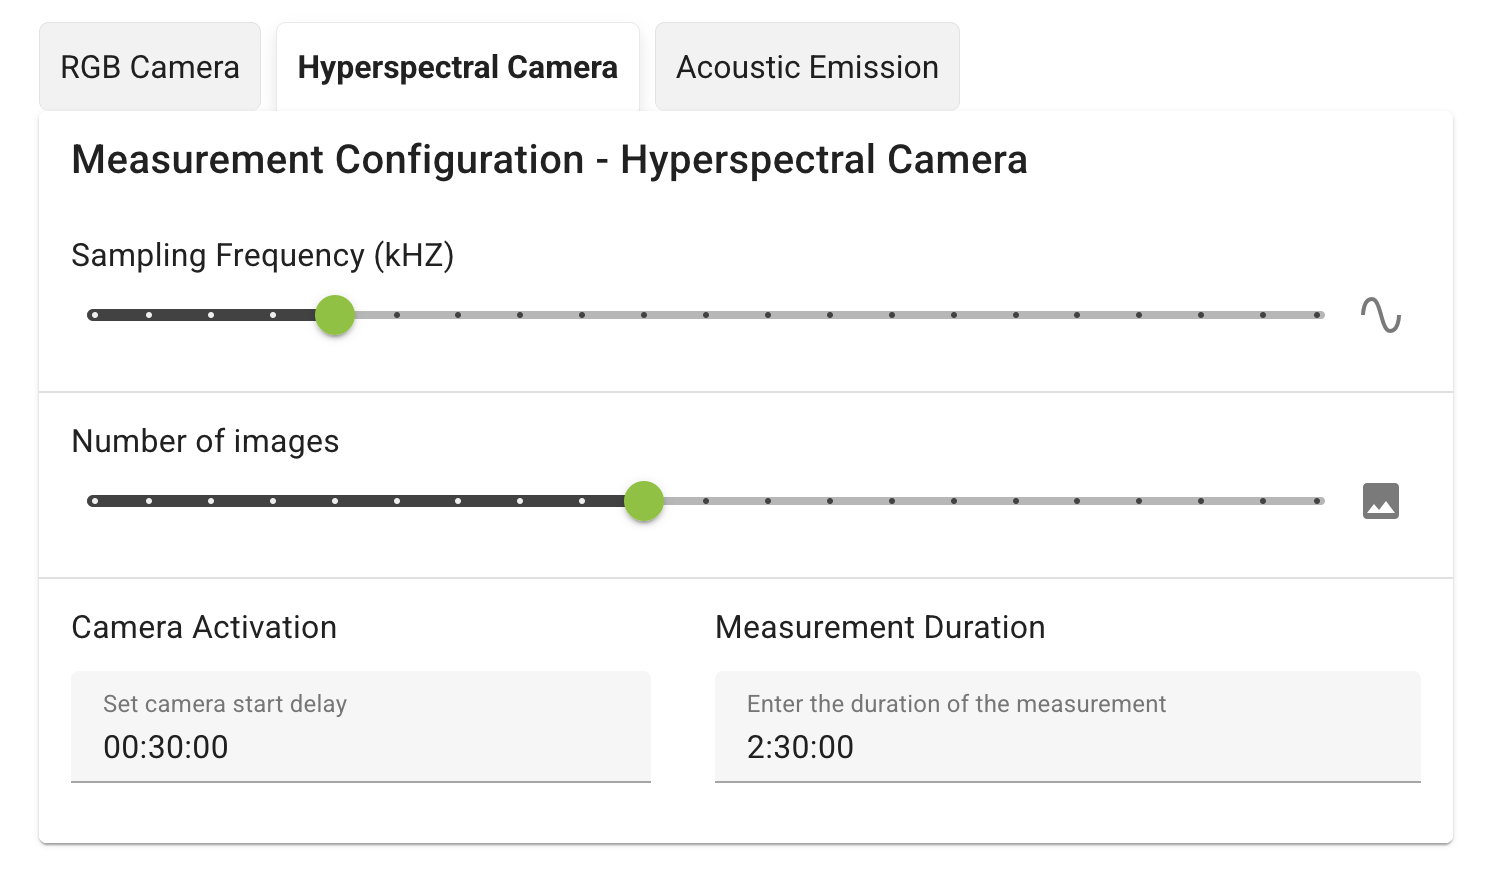
\includegraphics[width=0.7\textwidth]{../../img/multi_cam_settings}
            \caption{Tabulka pro nastavení multispektrální kamery}
            \label{fig:multi_cam_settings}
        \end{figure}

        \subsection{Akustická emise}\label{subsec:akusticka-emise}

        U zařízení na zaznamenávání akustických emisí je k dispozici nastavení vzorkovací frekvence, prahové hodnoty a doby
        definice vrcholu, které se provádí pohybem posuvníku vpravo nebo vlevo.
        Pod nimi se nachází okno pro nastavení
        doby, po kterou bude měření pomocí tohoto zařízení probíhat.

        \begin{figure}[hbt!]
            \centering
            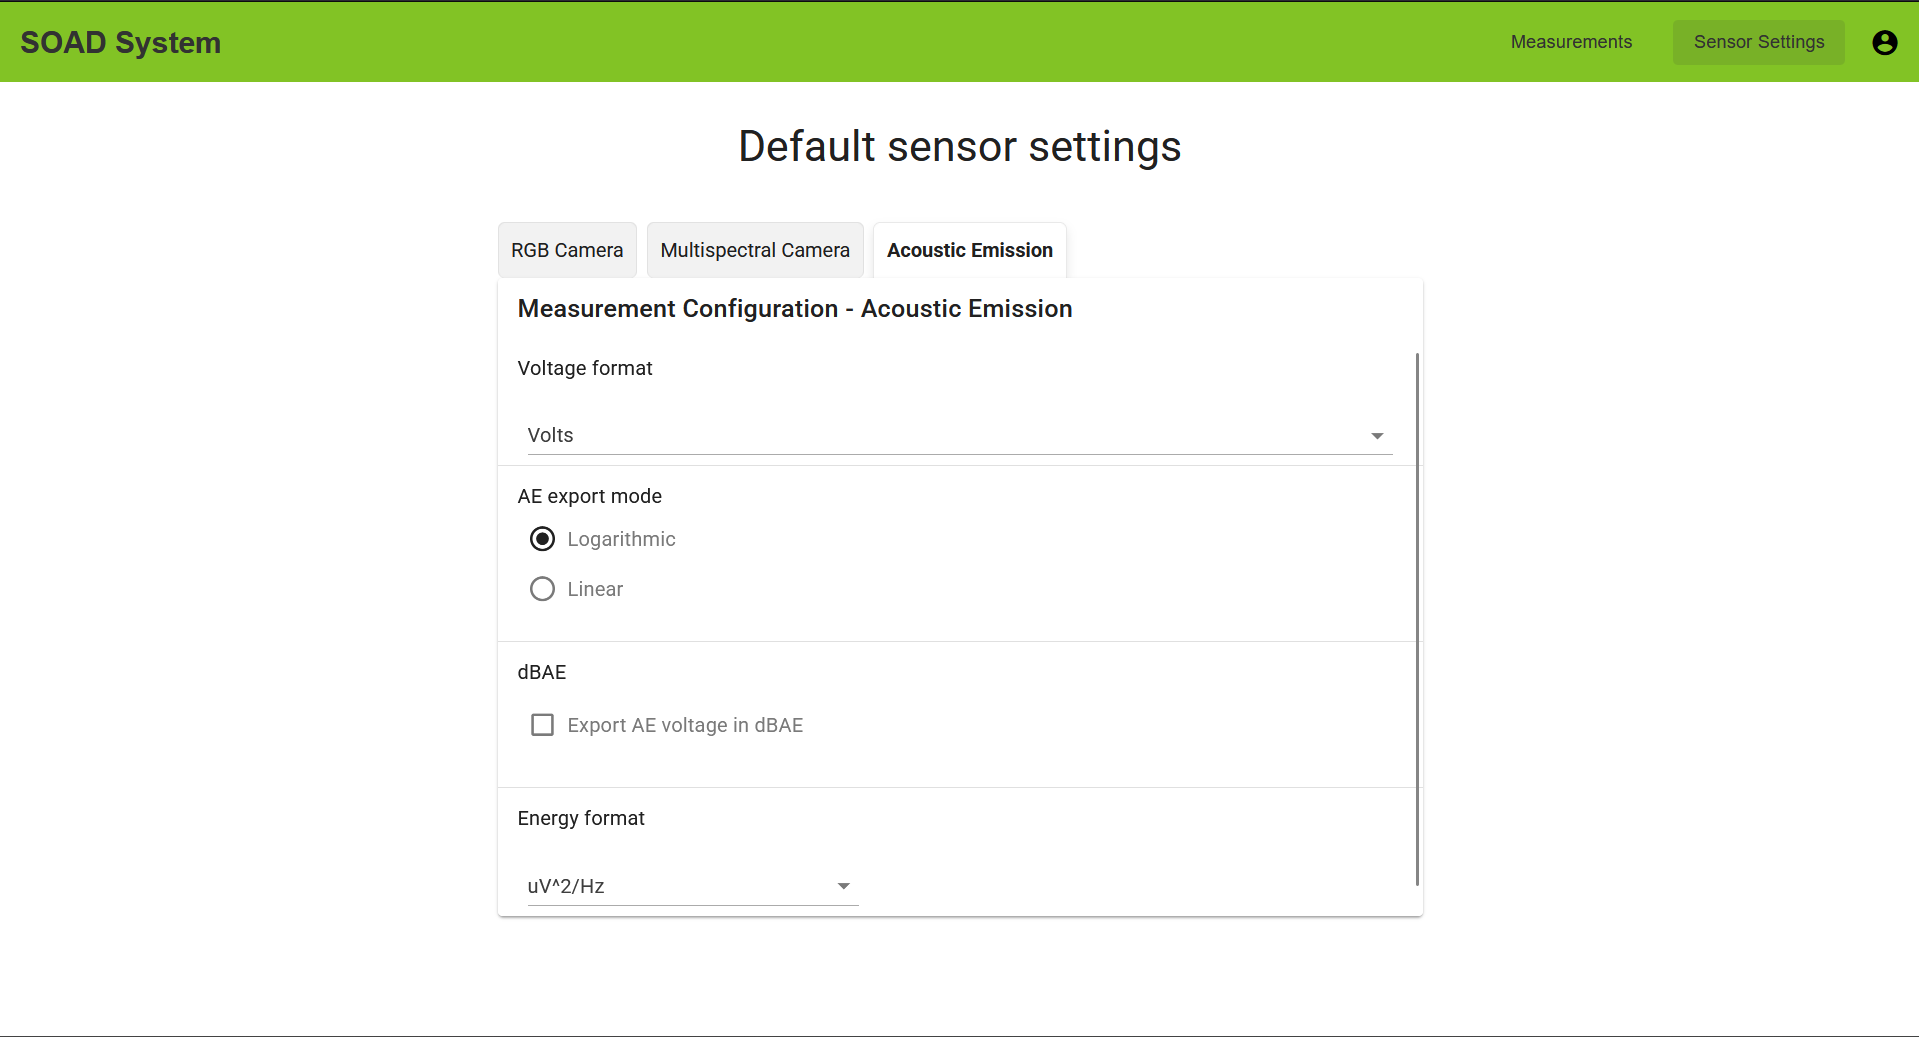
\includegraphics[width=0.8\textwidth]{../../img/ae_settings}
            \caption{Tabulka pro nastavení akustické emise}
            \label{fig:ae_settings}
        \end{figure}

        \subsection{Zahájení měření}\label{subsec:zahajeni-mereni}

        Měření se zahajuje na domovské stránce.
        Postup je následující:

        \begin{enumerate}
            \item Klikněte na tlačítko „MEASURE“, které se nachází v pravém horním rohu stránky (obrázek 6).
            \begin{figure}[hbt!]
                \centering
                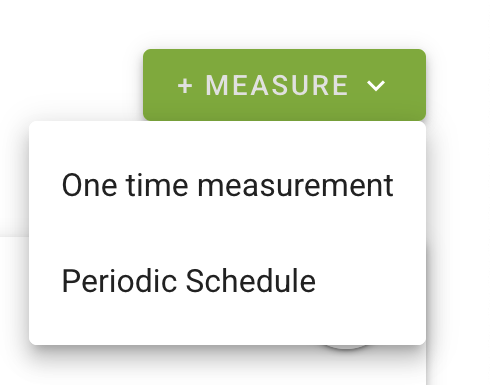
\includegraphics[width=0.32\textwidth]{../../img/measure_one_time_button}
                \caption{Tlačítko pro měření}
                \label{fig:measure_one_time}
            \end{figure}
            \item Z nabídky vyberte první variantu „One time measurement“
            \item V dialogovém okně uveďte název měření, popis a zvolte vhodný čas a parametry
            \begin{figure}[hbt!]
                  \centering
                  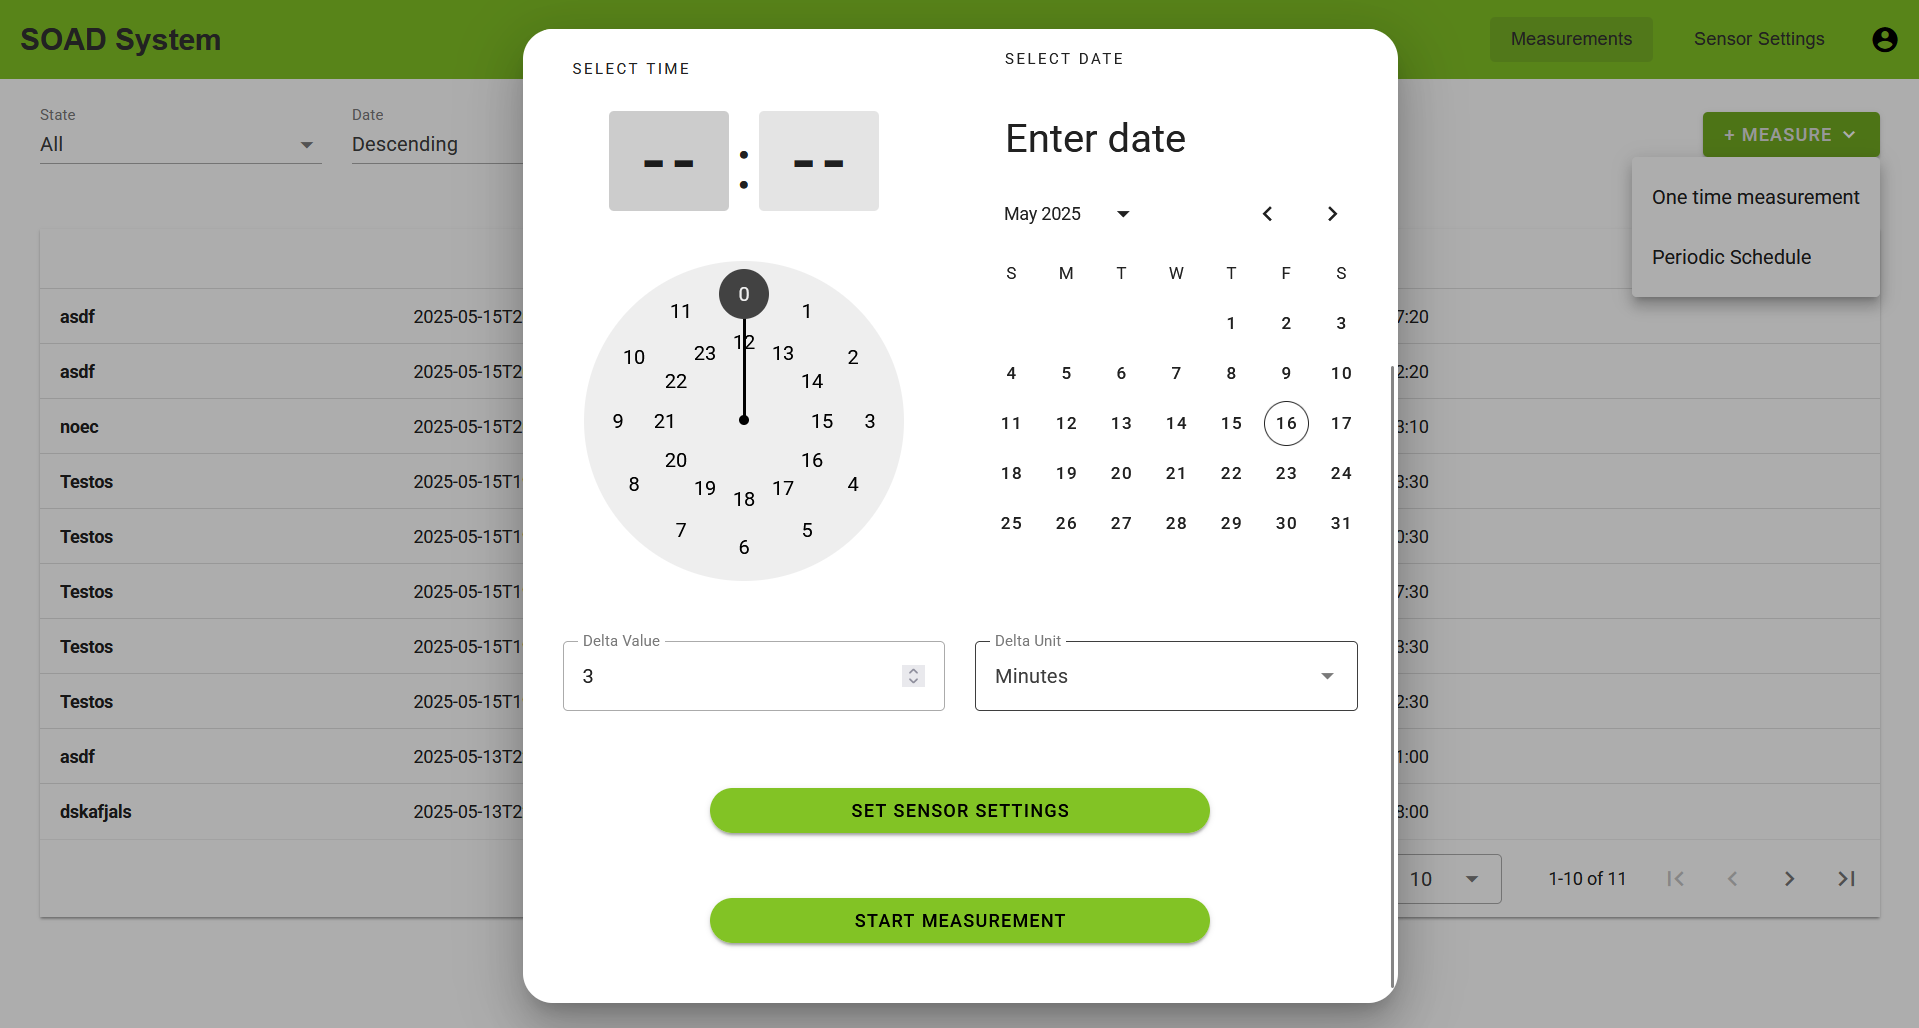
\includegraphics[width=0.8\textwidth]{../../img/one_time_measure_dialog}
                  \caption{Dialogové okno}
                  \label{fig:one_time_measure_dialog}
            \end{figure}
            \item Měření zahájíte kliknutím na tlačítko „START MEASUREMENT“ (na konci dialogu)
        \end{enumerate}

        Proces konfigurace periodického měření je podobný, pouze s tím rozdílem, že je třeba zvolit dva termíny.
        Pokud se měření nepodaří vytvořit, na konci dialogového okna bude zobrazeno upozornění.



        \subsection{Stahování dat}\label{subsec:stahovani-dat}

        Data k měření je možné stáhnout na hlavní stránce aplikace kliknutím na ikonu pro stažení u požadovaného záznamu.

        \begin{figure}[hbt!]
            \centering
            
\includegraphics[width=0.25\textwidth]{../../img/download_icon}
            \caption{Ikona pro stažení dat}
            \label{fig:dowload_icon}
        \end{figure}

    \end{teamwork}
\end{document}
